\documentclass[../../main.tex]{subfiles}

\begin{document}

\setchapterpreamble[u]{\margintoc}

\chapter{深度优先搜索和广度优先搜索}

深度优先搜索的本质是一种暴力搜索,我们从一个节点开始,不断地向下搜索,直到无法继续搜索为止。然后我们回溯到上一个节点,
继续搜索。通常这个回溯是通过递归的方式形成的,如果在搜索的过程中,我们需要记录搜索的节点,则我们需要伴随递归的自动
回溯对记录的数据进行删除和新增。

广度优先搜索的本质是一种暴力搜索,我们从一个节点开始,通过队列保存当前节点的所有子节点,然后不断地从队列中取出节点,
直到队列为空为止。

实际上,在树的章节中,我们已经使用过了很多次深度优先搜索和广度优先搜索的理念。

\section{带有回溯的简单的深度优先搜索}

\subsection{\href{https://leetcode.cn/problems/letter-combinations-of-a-phone-number/}{电话号码的字母组合}}
\label{subsec:letter-combinations-of-a-phone-number}


要解决这个问题,我们仍然需要把递归树画出来,如下图所示,我们列举出了数字2和3的所有的组合。我们可以发现,我们
需要维护一个字符串,然后不断地向下搜索,直到字符串的长度等于输入的字符串的长度。然后我们回溯到上一个节点,继续搜索。
同时,我们需要维持一个变量,记录当前的搜索的位置,用于修改当前字符串的值。

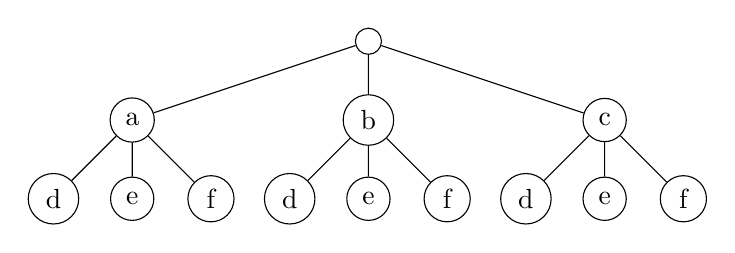
\begin{tikzpicture}[level distance=1cm,
  level 1/.style={sibling distance=3cm},
  level 2/.style={sibling distance=1cm}]
  \node[circle,draw] { }
    child {
      node[circle,draw] {a}
      child {
        node[circle,draw] {d}
      }
      child {
        node[circle,draw] {e}
      }
      child {
        node[circle,draw] {f}
      }
    }
    child {
      node[circle,draw] {b}
      child {
        node[circle,draw] {d}
      }
      child {
        node[circle,draw] {e}
      }
      child {
        node[circle,draw] {f}
      }
    }
    child {
      node[circle,draw] {c}
      child {
        node[circle,draw] {d}
      }
      child {
        node[circle,draw] {e}
      }
      child {
        node[circle,draw] {f}
      }
    };
\end{tikzpicture}

\lstinputlisting[language=C++]{code/letter-combinations-of-a-phone-number.cpp}

\subsection{\href{https://leetcode.cn/problems/generate-parentheses/}{括号生成}}

首先我们需要明确对于数字$n$总共有多少个左括号和右括号,我们可以发现,左括号的个数和右括号的个数都是$n$个。
同时,我们必须明确有效的含义:

\begin{itemize}
  \item 对于左括号而言,我们不需要做任何的检测,因为我们可以无限制的加入左括号直到$n$个。
  \item 对于右括号而言,当且仅当其数目小于左括号的数目时,我们才能够加入右括号。
\end{itemize}

我们可以使用深度优先搜索的思想,不断地向下搜索,直到左括号和右括号的数目都为$n$为止。我们需要维护一个字符串,
其大小为$2n$,然后不断地向下搜索,直到字符串的长度等于$2n$。然后我们回溯到上一个节点,继续搜索。同时,我们需要
维持两个变量,分别记录左括号和右括号的数目。

\lstinputlisting[language=C++]{code/generate-parentheses.cpp}

\subsection{\href{https://leetcode.cn/problems/combinations/}{组合}}

实际上这个题目和\ref{subsec:letter-combinations-of-a-phone-number}本质是一样的。我们需要实现一个
$1..n$的组合。同样地画出123组合两个数的递归树。同时我们可以实现一定的剪枝操作。

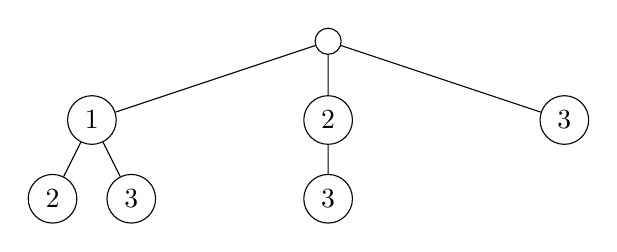
\begin{tikzpicture}[level distance=1cm,
  level 1/.style={sibling distance=3cm},
  level 2/.style={sibling distance=1cm}]
  \node[circle,draw] { }
    child {
      node[circle,draw] {1}
      child {
        node[circle,draw] {2}
      }
      child {
        node[circle,draw] {3}
      }
    }
    child {
      node[circle,draw] {2}
      child {
        node[circle,draw] {3}
      }
    }
    child {
      node[circle,draw] {3}
    };
\end{tikzpicture}

\lstinputlisting[language=C++]{code/combinations.cpp}

\end{document}
